\documentclass[11pt,a4paper]{article}
\usepackage[utf8]{inputenc}
\usepackage[T1]{fontenc}
\usepackage[margin=19mm]{geometry}
\usepackage{amsmath,graphicx,booktabs,array,longtable,caption}
\usepackage[hidelinks]{hyperref}
\setlength{\tabcolsep}{3pt}
\setlength{\parindent}{0pt}
\setlength{\parskip}{6pt}
\title{Technical report and complete balancing outcome atlas}
\author{Michael Agbo}
\date{12 November 2026}
\begin{document}
\maketitle
\section*{Purpose and main findings}
This technical report documents the numerical evidence supporting the accompanying manuscript. It preserves the complete torque-slice atlas, exact outcome counts, paired comparisons, controller settings, verification checks, and the distinction between completed and proposed experiments. It is intended to support independent review and reproduction.

The original study compares two fixed implementations on a nonlinear planar model. PID-type remains upright in 435 of 819 conditions but recovers position in only 215. LQR recovers in all 357 conditions where it stays upright. The 220 non-recovering PID-type survivors approach integral-dependent position offsets. Extending those cases to 30 s does not change their labels. Removing only the integral gain converts all 220 to recovery and adds two falls elsewhere.

\textbf{Outcome summary}
\begin{longtable}{p{0.324\linewidth}p{0.144\linewidth}p{0.144\linewidth}p{0.144\linewidth}p{0.144\linewidth}}
\toprule
Implementation & Recovered & Unsettled & Fallen & Total \\ \midrule \endhead
Original PID-type & 215 & 220 & 384 & 819 \\
Original LQR & 357 & 0 & 462 & 819 \\
PID-type with ki zero & 433 & 0 & 386 & 819 \\
\bottomrule
\end{longtable}
The ablation and horizon extension are post hoc analyses. They explain this implementation and do not establish a class-wide ranking. Counts are properties of a fixed parameter grid; no random sampling distribution, significance test, or binomial confidence interval is implied.

\section*{Study inventory}
\textbf{Completed numerical work}
\begin{longtable}{p{0.288\linewidth}p{0.162\linewidth}p{0.45\linewidth}}
\toprule
Analysis & Evaluations & Purpose \\ \midrule \endhead
Original grid & 1638 & Two fixed controllers on 819 shared conditions \\
Exact baseline reproduction & 1638 & All stored metric values verified at saved precision \\
Horizon extension & 220 & All original unsettled cases continued to 30 s \\
Integral ablation & 819 & ki changed from 0.4 to zero only \\
Refined integration & 705 & All boundary-adjacent cases at half physics step \\
Tolerance sensitivity & Reclassification & Final-window bounds applied to saved trajectories \\
\bottomrule
\end{longtable}
Baseline reproduction repeats the original trials and must not be counted as independent evidence. The refined integration audit repeats selected conditions with a changed numerical solver resolution. No additional physical robots, seeds, or sensor-noise realizations are implied by these totals.

\section*{Original outcome counts by torque limit}
\textbf{117 conditions per controller and torque limit}
\begin{longtable}{p{0.153\linewidth}p{0.207\linewidth}p{0.108\linewidth}p{0.108\linewidth}p{0.108\linewidth}p{0.216\linewidth}}
\toprule
Limit N m & Controller & R & U & F & Pre-push F \\ \midrule \endhead
0.1 & PID & 13 & 0 & 104 & 48 \\
0.1 & LQR & 5 & 0 & 112 & 48 \\
0.2 & PID & 31 & 4 & 82 & 0 \\
0.2 & LQR & 21 & 0 & 96 & 24 \\
0.3 & PID & 27 & 18 & 72 & 0 \\
0.3 & LQR & 45 & 0 & 72 & 0 \\
0.4 & PID & 27 & 36 & 54 & 0 \\
0.4 & LQR & 61 & 0 & 56 & 0 \\
0.5 & PID & 27 & 54 & 36 & 0 \\
0.5 & LQR & 63 & 0 & 54 & 0 \\
0.7 & PID & 45 & 54 & 18 & 0 \\
0.7 & LQR & 81 & 0 & 36 & 0 \\
1 & PID & 45 & 54 & 18 & 0 \\
1 & LQR & 81 & 0 & 36 & 0 \\
\bottomrule
\end{longtable}
R is recovered, U is upright but unsettled, and F is fallen. Pre-push F is a subset of F for trials with a planned nonzero push; the robot fell before any pulse was applied. Multiple planned push values can therefore correspond to the same initial-tilt failure. All such cases are retained in the stated Cartesian grid rather than silently removed.

\clearpage
\section*{Reproduction and numerical definitions}
The nominal model uses body mass 1.2 kg, translating base mass 0.35 kg, axle-to-body-centre distance 0.18 m, body-centre inertia 0.012 kg m\textsuperscript{2}, wheel radius 0.045 m, and each wheel inertia 0.00012 kg m\textsuperscript{2}. Translation and rotation drag are 0.08 N s/m and 0.002 N m s/rad. Gravity is 9.81 m/s\textsuperscript{2}. These values were not identified from hardware.

State order is x, v, theta, omega, with displacement in metres and angle in radians. The input is the total torque of both wheel motors. A force at the body centre enters translation and rotation. Gains are fixed across torque limits. The PID-type controller uses kp = 14, kd = 2, kx = 2, kv = 3, ki = 0.4, an integral clamp of 0.25 rad s, and conditional anti-windup. LQR uses Q = diag(12,2,120,2), R = 1 and the gain vector supplied in the archived configuration.

Each baseline run lasts at most 10 s, with a 0.2 s horizontal force pulse beginning at 2 s. Controls are held for 5 ms. RK4 integrates the plant. Fall detection is evaluated at control endpoints, at 45 degrees absolute tilt. Recovery requires a final dwell of at least one second within 1 degree tilt, 3 cm position, and 3 cm/s speed. For a nonzero pulse, recovery timing begins at 2.2 s; otherwise it begins at zero.

\section*{Linearization and integral state}
\textbf{PID-type augmented continuous poles}
\begin{longtable}{p{0.45\linewidth}p{0.45\linewidth}}
\toprule
Real part & Imaginary part \\ \midrule \endhead
-223.05302 & 0 \\
-7.8354457 & 0 \\
-0.98958498 & 0.65604438 \\
-0.98958498 & -0.65604438 \\
-3.222628e-15 & 0 \\
\bottomrule
\end{longtable}
The near-zero augmented mode corresponds to the equilibrium family x = -0.2 z. For the 220 continued cases, the largest 30 s difference between this predicted position and the unrounded numerical state is 2.76e-12 m. This is a consistency check inside the model, not a physical accuracy estimate. Stored rounded endpoint values in CSV are deliberately less precise than the raw state used for that residual.

\section*{Extended integration audit}
All 705 cells adjacent to a different outcome along tilt, force, or torque were recomputed with two physics substeps per 5 ms control interval. No controller update or event-detection interval was changed. There were 0 changes in the three-way outcome label. The maximum change in peak tilt was 3.8e-05 degrees. The complete audit records are included in data/full\_integration\_audit.json.

This is stronger than the original sampled 32-cell check, but it is still a finite numerical audit. It is not a formal error bound, an interval-arithmetic certificate, or proof of stability between grid points. Hardware-model mismatch is unaffected by refining the integrator.

\section*{Tests and provenance}
The baseline tests cover upright equilibrium, mechanical power balance, unforced energy conservation, RK4 convergence, parameter validation, local sampled LQR stability, nominal recovery, falls, anti-windup, and Python-to-JavaScript agreement. Sweep tests cover completeness, repeatability, nonmonotonic neighbouring outcomes, pre-push falls, report preservation, and fixed control timing under integration refinement. UI logic tests use mocked DOM and canvas objects; they are not a substitute for visual browser inspection.

The publication analysis additionally asserts equality of every stored baseline metric during reproduction and verifies that reclassification at the original 3 cm tolerance returns the original recovery counts. Analysis source hashes, the original result-file hash, configuration, and software versions are included in the package. Original model parameters and gains are preserved; the ablation is a separate configuration copy.

\section*{Paired recovering subset}
\textbf{Medians on 161 common recoveries}
\begin{longtable}{p{0.306\linewidth}p{0.162\linewidth}p{0.162\linewidth}p{0.27\linewidth}}
\toprule
Metric & PID-type & LQR & Paired LQR minus PID \\ \midrule \endhead
Recovery time s & 4.08 & 3.055 & -0.99 \\
Peak tilt deg & 10 & 10.559 & 0 \\
Max displacement m & 0.334092 & 0.299793 & -0.034299 \\
Squared torque integral & 0.010854 & 0.011967 & 0.001741 \\
\bottomrule
\end{longtable}
The final column is the median of paired differences, not the difference of two medians. Every condition that falls or fails recovery under either controller is excluded from this table. The exclusion must accompany any interpretation of response speed or effort.

\section*{Three-dimensional visualisations}
The companion visualisation/index.html displays six saved trajectories as orbitable three-dimensional robot schematics. Displacement, pitch and force timing are copied from the original trajectories. Wheel rotation uses the no-slip constraint. Display lanes separate the controllers; there is no lateral or yaw dynamics. The shell and track width are illustrative. A frozen final pose marks a fall rather than a simulated ground impact.

visualisation/experiments.html displays all 1,638 baseline records as discrete points in initial-tilt, push-force and torque-limit space, with controller, outcome and torque-slice filters. It does not interpolate a stability surface. The static figure below displays selected paths in state space; the animated GIF supplies a browser-independent robot preview. Interactive WebGL rendering could not be visually inspected because the browser access host was unavailable. Automated checks verify exact replay data, sample selection, centre-of-mass mapping, force timing and outcome totals.

\begin{figure}[htbp]
\centering
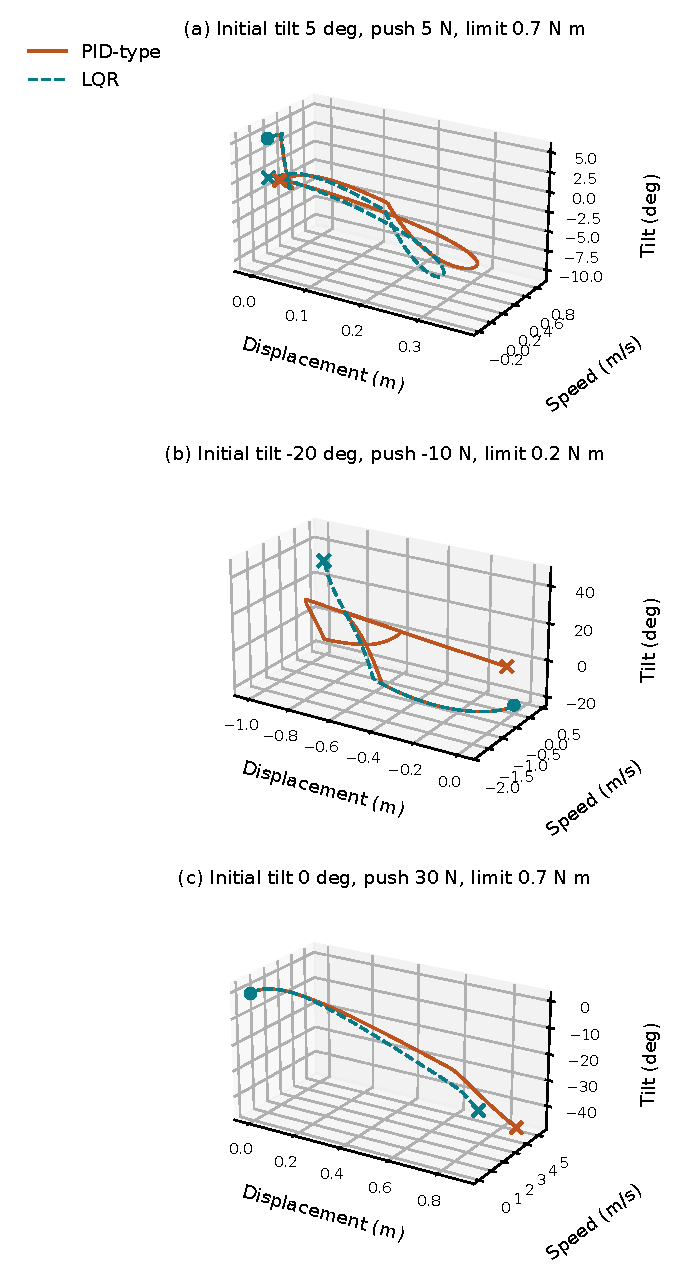
\includegraphics[width=\linewidth,height=.65\textheight,keepaspectratio]{../../figures/fig09_3d_state_trajectories.pdf}
\caption{Three-dimensional state trajectories in displacement, speed and tilt for three explicitly selected examples. Solid orange: PID-type; dashed teal: LQR. Circles mark initial states and crosses final states. Paths stop at 10 s or the declared fall, with no ground-impact extrapolation. These are planar-model state-space curves, not three-dimensional rigid-body motion; each panel uses its own axis scale.}
\end{figure}
\clearpage
\section*{Complete outcome atlas}
These seven torque slices show every original condition. Axes and symbol meanings are identical across slices. No interpolation or fitted boundary is used. A listed recovered force at zero initial tilt is an evaluated value only; it is not a guaranteed disturbance threshold.

\section*{Torque slice 0.1 N m}
\begin{figure}[htbp]
\centering
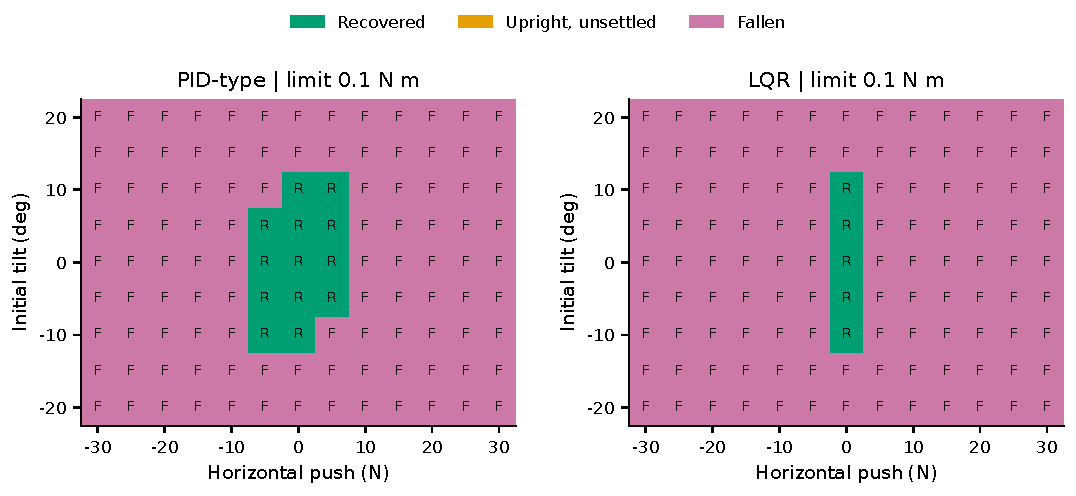
\includegraphics[width=\linewidth,height=.65\textheight,keepaspectratio]{../../figures/sfig01_torque_0p1.pdf}
\caption{Complete paired outcome maps at a total torque limit of 0.1 N m. Each map contains 117 conditions. R, U, and F label recovery, upright non-recovery, and fall respectively. Each trial has exact measurements and the same nominal body parameters.}
\end{figure}
PID recovered at zero initial tilt for these tested force values: -5 N, 0 N, 5 N.

LQR recovered at zero initial tilt for these tested force values: 0 N.

\textbf{Slice summary}
\begin{longtable}{p{0.252\linewidth}p{0.108\linewidth}p{0.108\linewidth}p{0.108\linewidth}p{0.324\linewidth}}
\toprule
Controller & R & U & F & Largest travel m \\ \midrule \endhead
PID & 13 & 0 & 104 & 0.535 \\
LQR & 5 & 0 & 112 & 0.447 \\
\bottomrule
\end{longtable}
Every slice contains 117 conditions for each controller. Larger travel is not penalized directly by the fall label; the operational position criterion applies to the final dwell. Conditions with early falls can be duplicated across planned forces because the pulse is scheduled after the initial balancing transient.

\clearpage
\section*{Torque slice 0.2 N m}
\begin{figure}[htbp]
\centering
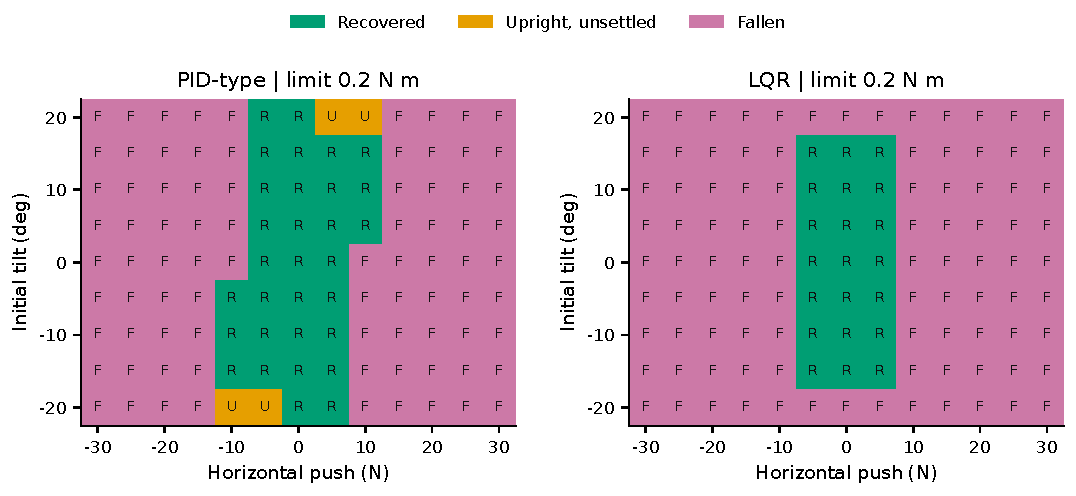
\includegraphics[width=\linewidth,height=.65\textheight,keepaspectratio]{../../figures/sfig02_torque_0p2.pdf}
\caption{Complete paired outcome maps at a total torque limit of 0.2 N m. Each map contains 117 conditions. R, U, and F label recovery, upright non-recovery, and fall respectively. Each trial has exact measurements and the same nominal body parameters.}
\end{figure}
PID recovered at zero initial tilt for these tested force values: -5 N, 0 N, 5 N.

LQR recovered at zero initial tilt for these tested force values: -5 N, 0 N, 5 N.

\textbf{Slice summary}
\begin{longtable}{p{0.252\linewidth}p{0.108\linewidth}p{0.108\linewidth}p{0.108\linewidth}p{0.324\linewidth}}
\toprule
Controller & R & U & F & Largest travel m \\ \midrule \endhead
PID & 31 & 4 & 82 & 1.460 \\
LQR & 21 & 0 & 96 & 1.108 \\
\bottomrule
\end{longtable}
Every slice contains 117 conditions for each controller. Larger travel is not penalized directly by the fall label; the operational position criterion applies to the final dwell. Conditions with early falls can be duplicated across planned forces because the pulse is scheduled after the initial balancing transient.

\clearpage
\section*{Torque slice 0.3 N m}
\begin{figure}[htbp]
\centering
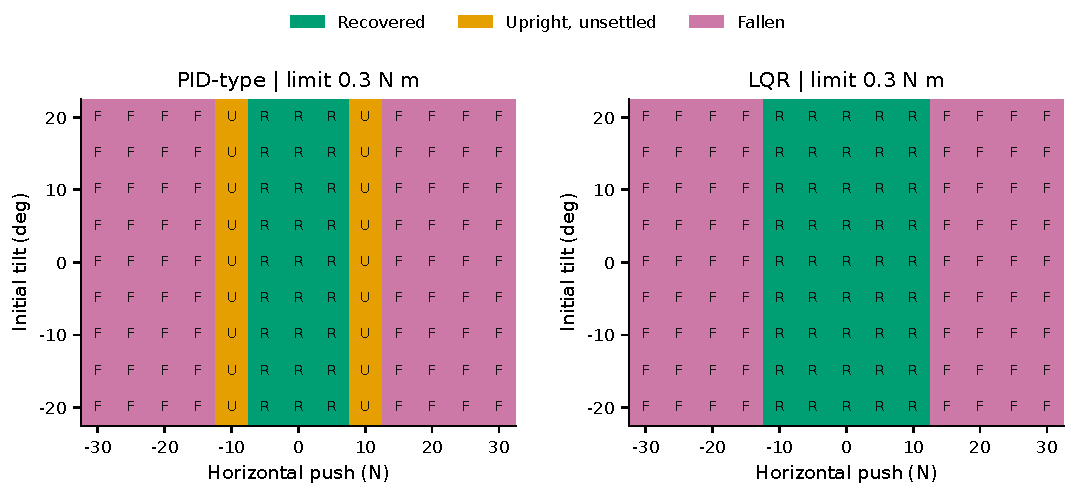
\includegraphics[width=\linewidth,height=.65\textheight,keepaspectratio]{../../figures/sfig03_torque_0p3.pdf}
\caption{Complete paired outcome maps at a total torque limit of 0.3 N m. Each map contains 117 conditions. R, U, and F label recovery, upright non-recovery, and fall respectively. Each trial has exact measurements and the same nominal body parameters.}
\end{figure}
PID recovered at zero initial tilt for these tested force values: -5 N, 0 N, 5 N.

LQR recovered at zero initial tilt for these tested force values: -10 N, -5 N, 0 N, 5 N, 10 N.

\textbf{Slice summary}
\begin{longtable}{p{0.252\linewidth}p{0.108\linewidth}p{0.108\linewidth}p{0.108\linewidth}p{0.324\linewidth}}
\toprule
Controller & R & U & F & Largest travel m \\ \midrule \endhead
PID & 27 & 18 & 72 & 3.446 \\
LQR & 45 & 0 & 72 & 3.519 \\
\bottomrule
\end{longtable}
Every slice contains 117 conditions for each controller. Larger travel is not penalized directly by the fall label; the operational position criterion applies to the final dwell. Conditions with early falls can be duplicated across planned forces because the pulse is scheduled after the initial balancing transient.

\clearpage
\section*{Torque slice 0.4 N m}
\begin{figure}[htbp]
\centering
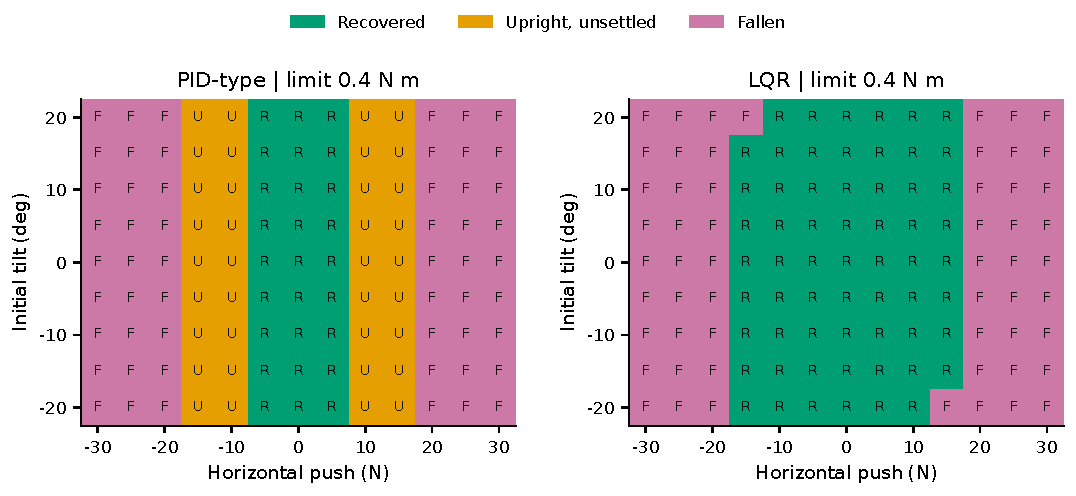
\includegraphics[width=\linewidth,height=.65\textheight,keepaspectratio]{../../figures/sfig04_torque_0p4.pdf}
\caption{Complete paired outcome maps at a total torque limit of 0.4 N m. Each map contains 117 conditions. R, U, and F label recovery, upright non-recovery, and fall respectively. Each trial has exact measurements and the same nominal body parameters.}
\end{figure}
PID recovered at zero initial tilt for these tested force values: -5 N, 0 N, 5 N.

LQR recovered at zero initial tilt for these tested force values: -15 N, -10 N, -5 N, 0 N, 5 N, 10 N, 15 N.

\textbf{Slice summary}
\begin{longtable}{p{0.252\linewidth}p{0.108\linewidth}p{0.108\linewidth}p{0.108\linewidth}p{0.324\linewidth}}
\toprule
Controller & R & U & F & Largest travel m \\ \midrule \endhead
PID & 27 & 36 & 54 & 1.686 \\
LQR & 61 & 0 & 56 & 1.634 \\
\bottomrule
\end{longtable}
Every slice contains 117 conditions for each controller. Larger travel is not penalized directly by the fall label; the operational position criterion applies to the final dwell. Conditions with early falls can be duplicated across planned forces because the pulse is scheduled after the initial balancing transient.

\clearpage
\section*{Torque slice 0.5 N m}
\begin{figure}[htbp]
\centering
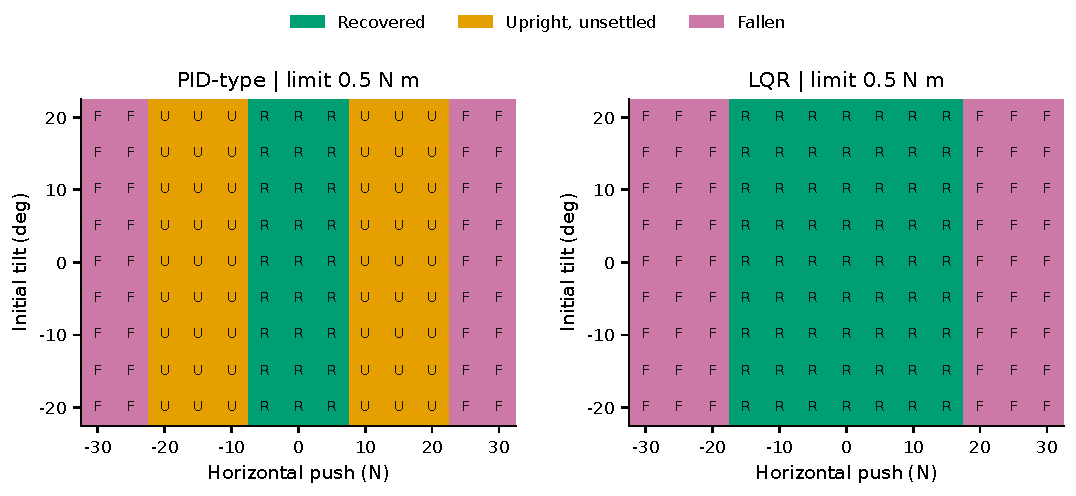
\includegraphics[width=\linewidth,height=.65\textheight,keepaspectratio]{../../figures/sfig05_torque_0p5.pdf}
\caption{Complete paired outcome maps at a total torque limit of 0.5 N m. Each map contains 117 conditions. R, U, and F label recovery, upright non-recovery, and fall respectively. Each trial has exact measurements and the same nominal body parameters.}
\end{figure}
PID recovered at zero initial tilt for these tested force values: -5 N, 0 N, 5 N.

LQR recovered at zero initial tilt for these tested force values: -15 N, -10 N, -5 N, 0 N, 5 N, 10 N, 15 N.

\textbf{Slice summary}
\begin{longtable}{p{0.252\linewidth}p{0.108\linewidth}p{0.108\linewidth}p{0.108\linewidth}p{0.324\linewidth}}
\toprule
Controller & R & U & F & Largest travel m \\ \midrule \endhead
PID & 27 & 54 & 36 & 1.398 \\
LQR & 63 & 0 & 54 & 1.021 \\
\bottomrule
\end{longtable}
Every slice contains 117 conditions for each controller. Larger travel is not penalized directly by the fall label; the operational position criterion applies to the final dwell. Conditions with early falls can be duplicated across planned forces because the pulse is scheduled after the initial balancing transient.

\clearpage
\section*{Torque slice 0.7 N m}
\begin{figure}[htbp]
\centering
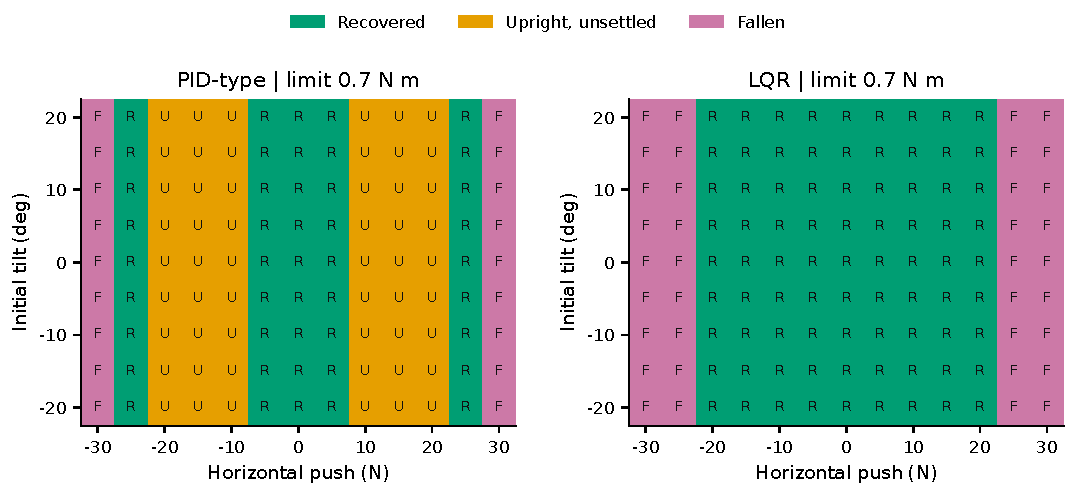
\includegraphics[width=\linewidth,height=.65\textheight,keepaspectratio]{../../figures/sfig06_torque_0p7.pdf}
\caption{Complete paired outcome maps at a total torque limit of 0.7 N m. Each map contains 117 conditions. R, U, and F label recovery, upright non-recovery, and fall respectively. Each trial has exact measurements and the same nominal body parameters.}
\end{figure}
PID recovered at zero initial tilt for these tested force values: -25 N, -5 N, 0 N, 5 N, 25 N.

LQR recovered at zero initial tilt for these tested force values: -20 N, -15 N, -10 N, -5 N, 0 N, 5 N, 10 N, 15 N, 20 N.

\textbf{Slice summary}
\begin{longtable}{p{0.252\linewidth}p{0.108\linewidth}p{0.108\linewidth}p{0.108\linewidth}p{0.324\linewidth}}
\toprule
Controller & R & U & F & Largest travel m \\ \midrule \endhead
PID & 45 & 54 & 18 & 1.663 \\
LQR & 81 & 0 & 36 & 1.128 \\
\bottomrule
\end{longtable}
Every slice contains 117 conditions for each controller. Larger travel is not penalized directly by the fall label; the operational position criterion applies to the final dwell. Conditions with early falls can be duplicated across planned forces because the pulse is scheduled after the initial balancing transient.

\clearpage
\section*{Torque slice 1 N m}
\begin{figure}[htbp]
\centering
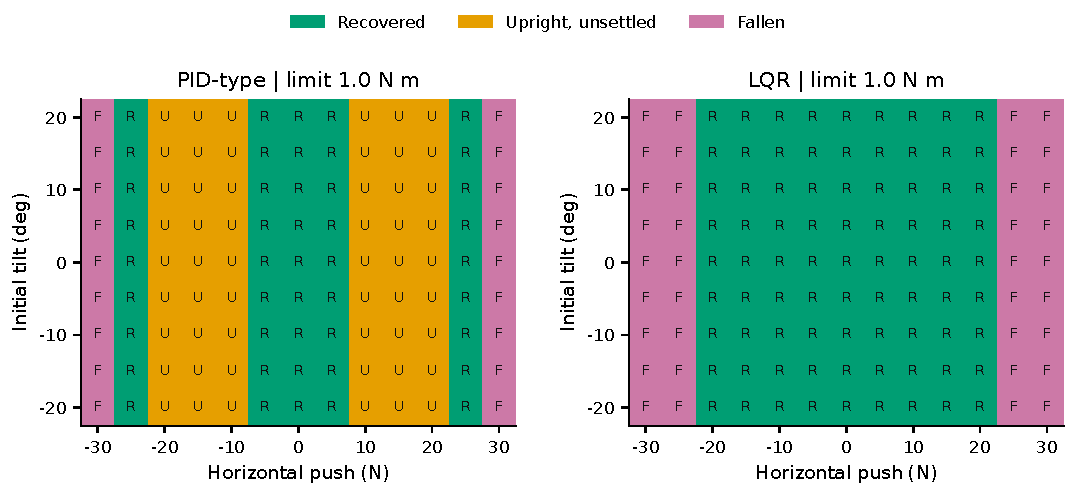
\includegraphics[width=\linewidth,height=.65\textheight,keepaspectratio]{../../figures/sfig07_torque_1p0.pdf}
\caption{Complete paired outcome maps at a total torque limit of 1 N m. Each map contains 117 conditions. R, U, and F label recovery, upright non-recovery, and fall respectively. Each trial has exact measurements and the same nominal body parameters.}
\end{figure}
PID recovered at zero initial tilt for these tested force values: -25 N, -5 N, 0 N, 5 N, 25 N.

LQR recovered at zero initial tilt for these tested force values: -20 N, -15 N, -10 N, -5 N, 0 N, 5 N, 10 N, 15 N, 20 N.

\textbf{Slice summary}
\begin{longtable}{p{0.252\linewidth}p{0.108\linewidth}p{0.108\linewidth}p{0.108\linewidth}p{0.324\linewidth}}
\toprule
Controller & R & U & F & Largest travel m \\ \midrule \endhead
PID & 45 & 54 & 18 & 1.660 \\
LQR & 81 & 0 & 36 & 1.126 \\
\bottomrule
\end{longtable}
Every slice contains 117 conditions for each controller. Larger travel is not penalized directly by the fall label; the operational position criterion applies to the final dwell. Conditions with early falls can be duplicated across planned forces because the pulse is scheduled after the initial balancing transient.

\clearpage
\section*{Steps 3 and 4 and the submission pathway}
The current material is a journal-neutral manuscript draft and a reproducible simulation package. It has not established a new general control method, hardware validity, or superiority after matched tuning. Before selecting a submission venue, the author should decide whether the intended contribution is an evaluation methodology, a new estimator or controller, or a validated robotics implementation. Additional features alone do not establish novelty.

\section*{Step 3 Imperfect measurements}
Begin with a measurement model defined independently from the true simulated state. Introduce angular measurement noise and gyro noise separately, then introduce observation delay through an explicit history buffer. Keep force timing and controller period fixed. Label a simple angular-noise surrogate as such; a physical accelerometer model must also account for translational acceleration and orientation. A complementary or Kalman estimator should use only past and present measurements.

Select conditions near and away from the present boundaries before examining noisy outcomes. Use common random-number seeds across controllers where the disturbance model permits, and preserve individual trials. An initial design could use at least 30 independent noise realizations per stochastic condition, with more trials where interval width remains large. Report fall frequency with an appropriate binomial interval for independent repeats of a fixed condition, plus recovery and estimator error. Do not apply those intervals to the present deterministic grid.

\section*{Step 4 Physically consistent payload variation}
Start with static payloads present at initialization. For a payload mass mp at vertical distance lp from the axle, update total body mass to m + mp and centre distance to (m l + mp lp)/(m + mp). Recompute body inertia with the parallel-axis theorem, including the payload inertia. Lateral offsets require a changed equilibrium orientation and a correspondingly consistent gravitational model; they cannot be represented by changing mass alone.

First hold the original gains fixed to characterize robustness. Compare retuned or adaptive controllers only in a separate, transparently specified experiment. Distinguish calibration conditions from held-out tests. A sudden load pickup requires an explicit treatment of the initial state and momentum exchange; it is not equivalent to silently replacing parameters during an integration step. Only after separate sensing and payload studies should their interaction be tested.

\section*{Work needed before submission}
\textbf{Development priorities}
\begin{longtable}{p{0.108\linewidth}p{0.288\linewidth}p{0.504\linewidth}}
\toprule
Priority & Deliverable & Evidence required \\ \midrule \endhead
1 & Fair baseline comparison & Matched tuning objective or budget, several gain sets, and held-out conditions \\
2 & Independent model validation & Cross-check with another simulator or identified hardware response \\
3 & Sensing and delay study & Explicit measurement model, estimator, seeds, uncertainty summaries \\
4 & Payload study & Consistent mass properties, frozen-gain and redesigned-gain comparisons \\
5 & Contribution and related work & A narrow novelty statement supported by a deeper literature review \\
6 & Reproducible release & Reviewed code, frozen environment, data archive, and persistent identifier \\
\bottomrule
\end{longtable}
No external submission, repository publication, data upload, or claim of peer review has been made. Michael Agbo should review and approve the scientific content, authorship details, affiliation, declarations, and final venue requirements. AI-assisted coding and drafting should be disclosed according to the selected venue policy.

\section*{References}
[1] L. B. Lau, N. S. Ahmad, and P. Goh. Self-balancing robot: modeling and comparative analysis between PID and linear quadratic regulator. International Journal of Reconfigurable and Embedded Systems 12(3), 351-359, 2023. \url{https://doi.org/10.11591/ijres.v12.i3.pp351-359}\par
[2] K. Laddach, M. Czyzniewski, and R. Langowski. A selection of PID type controller settings via LQR approach for two-wheeled balancing robot. 2021 25th International Conference on Methods and Models in Automation and Robotics, 378-383, 2021. \url{https://doi.org/10.1109/MMAR49549.2021.9528471}\par
[3] K. Albert, K. S. Phogat, F. Anhalt, R. N. Banavar, D. Chatterjee, and B. Lohmann. Structure-Preserving Constrained Optimal Trajectory Planning of a Wheeled Inverted Pendulum. arXiv:1811.12819v2, 2019. Preprint version. \url{https://arxiv.org/abs/1811.12819v2}\par
[4] Z. Music, F. Molinari, S. Gallenmuller, O. Ayan, S. Zoppi, W. Kellerer, G. Carle, T. Seel, and J. Raisch. Design of a Networked Controller for a Two-Wheeled Inverted Pendulum Robot. arXiv:1812.03071v2, 2019. Preprint version; related publication DOI 10.1016/j.ifacol.2019.12.153. \url{https://arxiv.org/abs/1812.03071v2}\par
[5] D. Baek, Y. Sim, A. Purushottam, S. Gupta, and J. Ramos. Toward Control of Wheeled Humanoid Robots with Unknown Payloads: Equilibrium Point Estimation via Real-to-Sim Adaptation. arXiv:2403.10948v2, 2024. Preprint. \url{https://arxiv.org/abs/2403.10948v2}\par
[6] Y. Song, G. Wan, and X. Cao. Gain-Scheduled Control of a Wheeled Inverted-Pendulum Robot with Load-Induced Equilibrium Drift Compensation. Applied Sciences 16(10), 4876, 2026. \url{https://doi.org/10.3390/app16104876}\par
\end{document}
